This chapter contains the detailed design of the emitter satellite. Each section contains the final design of a different subsystem. 
\\\\
The most important subsystem is the optical emitting payload which can found in section \ref{sec:DDlaser}. The navigation and satellite position is discussed in section \ref{NaviEmitter}. Thirdly the inter-satellite and space-ground communication is explained in detail in section \ref{sec:comm_emitter}. Section \ref{emDDadcs} contains the detailed design of the \ac{ADCS}. The power generation and the corresponding power system is documented in section \ref{emitter_EPS}. The emitter satellite also has a \ac{SPAD} instrument. The details can be found in section \ref{sec:DDreceiver}.
\\\\
Figure \ref{fig:emitterSat} shows an impression of what the emitter satellite will look like.

\begin{figure}
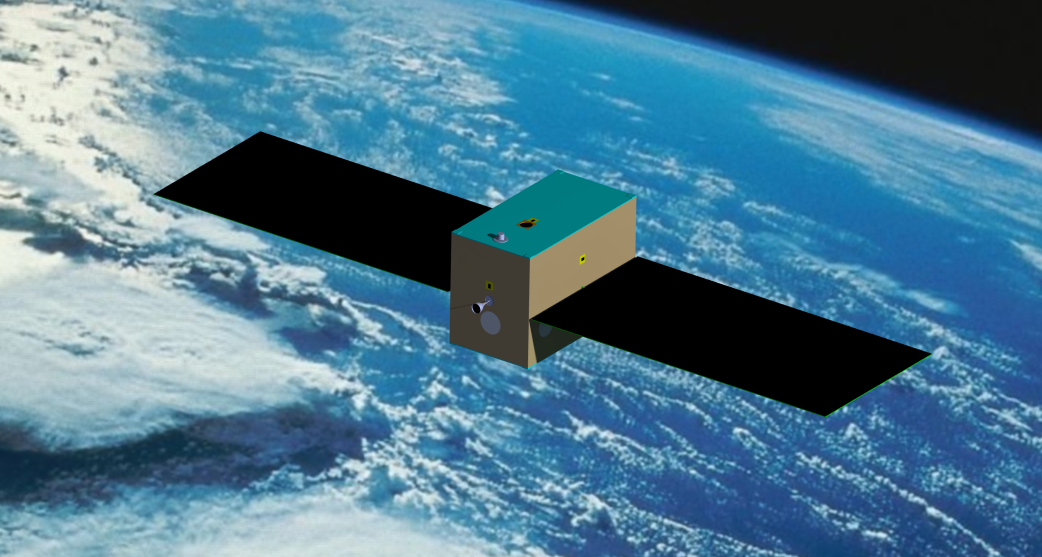
\includegraphics{chapters/img/emitter.tif}
\caption{Impression of the emitter satellite}
\label{fig:emitterSat}
\end{figure}